\documentclass[11pt]{article}
\usepackage[utf8]{inputenc}
\usepackage[T1]{fontenc}
\usepackage{amsmath}
\usepackage{multicol}
\usepackage{geometry}
\usepackage{tikz}
\usetikzlibrary{shapes.geometric, arrows.meta, angles, quotes, calc}
\usepackage{enumitem}
\usepackage{xcolor}
\usepackage{titlesec}
\usepackage{parskip}
\setlength{\parskip}{0.5em}
\renewcommand{\baselinestretch}{1.0}

% Configurações de layout
\geometry{a4paper, left=1cm, right=1cm, top=0.5cm, bottom=1.2cm}
\setlength{\columnseprule}{0.4pt}
\setlength{\baselineskip}{1.0\baselineskip}

% Cores para títulos
\titleformat{\section}{\normalfont\Large\bfseries\color{blue}}{\thesection}{1em}{}
\titleformat{\subsection}{\normalfont\large\bfseries\color{red}}{\thesubsection}{1em}{}
\titleformat{\subsubsection}{\normalfont\normalsize\bfseries\color{black}}{\thesubsubsection}{1em}{}

\title{\textcolor{blue}{Geometria Plana: Triângulos \\ Congruência, Semelhança e Trigonometria}}
\author{Professor: Jefferson}
\date{}

\begin{document}

\maketitle
\vspace{-1cm}

\begin{center}
    \large{Nome: \underline{\hspace{8cm}} \quad Turma: \underline{\hspace{3cm}}}
\end{center}

\begin{multicols}{2}

\section*{1. Congruência de Triângulos}

Dois triângulos são \textbf{congruentes} quando têm os três lados e os três ângulos respectivamente congruentes.

\subsection*{Casos de Congruência}
\begin{itemize}
    \item \textbf{LAL} (Lado-Ângulo-Lado): Dois lados e o ângulo entre eles
    \item \textbf{ALA} (Ângulo-Lado-Ângulo): Dois ângulos e o lado entre eles
    \item \textbf{LLL} (Lado-Lado-Lado): Três lados
    \item \textbf{LAA} (Lado-Ângulo-Ângulo): Um lado e dois ângulos adjacentes
\end{itemize}

\begin{center}
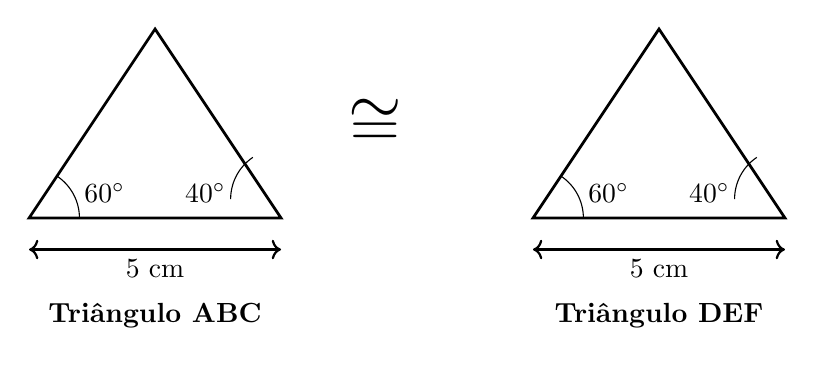
\begin{tikzpicture}[scale=0.8]  % Aumentei de 0.6 para 0.8
% Triângulo 1
\begin{scope}
\draw[thick, line width=1pt] (0,0) -- (4,0) -- (2,3) -- cycle;  % Aumentei as dimensões
\draw[<->, line width=0.8pt] (0,-0.5) -- (4,-0.5) node[midway,below] {5 cm};  % Aumentei o espaçamento
\draw (0.8,0) arc (0:56:0.8);  % Aumentei o raio do arco
\node at (1.2,0.4) {$60^\circ$};  % Ajustei a posição
\draw (3.2,0.3) arc (180:124:0.8);  % Aumentei o raio do arco
\node at (2.8,0.4) {$40^\circ$};  % Ajustei a posição
\node[below] at (2,-1.2) {\textbf{Triângulo ABC}};  % Melhorei a legenda
\end{scope}

% Seta de congruência - aumentei o tamanho
\begin{scope}[xshift=5.5cm]  % Aumentei o espaçamento
\node at (0,1.5) {\Huge $\cong$};  % Aumentei o símbolo
\end{scope}

% Triângulo 2
\begin{scope}[xshift=8cm]  % Aumentei o espaçamento
\draw[thick, line width=1pt] (0,0) -- (4,0) -- (2,3) -- cycle;  % Aumentei as dimensões
\draw[<->, line width=0.8pt] (0,-0.5) -- (4,-0.5) node[midway,below] {5 cm};  % Aumentei o espaçamento
\draw (0.8,0) arc (0:56:0.8);  % Aumentei o raio do arco
\node at (1.2,0.4) {$60^\circ$};  % Ajustei a posição
\draw (3.2,0.3) arc (180:124:0.8);  % Aumentei o raio do arco
\node at (2.8,0.4) {$40^\circ$};  % Ajustei a posição
\node[below] at (2,-1.2) {\textbf{Triângulo DEF}};  % Melhorei a legenda
\end{scope}
\end{tikzpicture}
\end{center}
\subsection*{Exercícios de Congruência}
\begin{enumerate}
    \item Determine se os triângulos são congruentes:
    \begin{enumerate}[label=\alph*)]
        \item Lados: 5 cm, 6 cm, 7 cm e 5 cm, 6 cm, 7 cm
        \item Lados: 4 cm, 5 cm, 6 cm e 5 cm, 4 cm, 6 cm
        \item Ângulos: $30^\circ$, $60^\circ$, $90^\circ$ e $60^\circ$, $30^\circ$, $90^\circ$
    \end{enumerate}
    
    \item Complete com o caso de congruência:
    \begin{enumerate}[label=\alph*)]
        \item AB = DE, BC = EF, $\angle B = \angle E$: \underline{\hspace{2cm}}
        \item $\angle A = \angle D$, $\angle B = \angle E$, AB = DE: \underline{\hspace{2cm}}
        \item AB = DE, BC = EF, AC = DF: \underline{\hspace{2cm}}
    \end{enumerate}
\end{enumerate}

\section*{2. Semelhança de Triângulos}

Dois triângulos são \textbf{semelhantes} quando têm os ângulos respectivamente congruentes e os lados correspondentes proporcionais.

\subsection*{Casos de Semelhança}
\begin{itemize}
    \item \textbf{AA} (Ângulo-Ângulo): Dois ângulos congruentes
    \item \textbf{LAL} (Lado-Ângulo-Lado): Dois lados proporcionais e o ângulo entre congruente
    \item \textbf{LLL} (Lado-Lado-Lado): Três lados proporcionais
\end{itemize}

\begin{center}
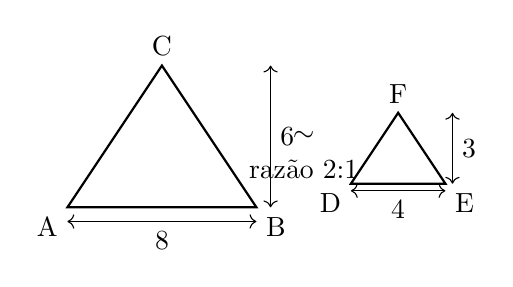
\begin{tikzpicture}[scale=0.6]
% Triângulo maior
\begin{scope}
\draw[thick] (0,0) -- (4,0) -- (2,3) -- cycle;
\node[below left] at (0,0) {A};
\node[below right] at (4,0) {B};
\node[above] at (2,3) {C};
\draw[<->] (0,-0.3) -- (4,-0.3) node[midway,below] {8};
\draw[<->] (4.3,0) -- (4.3,3) node[midway,right] {6};
\end{scope}

% Triângulo menor
\begin{scope}[xshift=6cm, yshift=0.5cm, scale=0.5]
\draw[thick] (0,0) -- (4,0) -- (2,3) -- cycle;
\node[below left] at (0,0) {D};
\node[below right] at (4,0) {E};
\node[above] at (2,3) {F};
\draw[<->] (0,-0.3) -- (4,-0.3) node[midway,below] {4};
\draw[<->] (4.3,0) -- (4.3,3) node[midway,right] {3};
\end{scope}

% Razão
\node at (5,1.5) {$\sim$};
\node at (5,0.8) {razão 2:1};
\end{tikzpicture}
\end{center}

\subsection*{Relações em Triângulos Semelhantes}
Se $\triangle ABC \sim \triangle DEF$, então:
\begin{itemize}
    \item $\dfrac{AB}{DE} = \dfrac{BC}{EF} = \dfrac{AC}{DF} = k$
    \item $\dfrac{h_1}{h_2} = k$ (razão das alturas)
    \item $\dfrac{A_1}{A_2} = k^2$ (razão das áreas)
\end{itemize}

\subsection*{Exercícios de Semelhança}
\begin{enumerate}
    \item Calcule $x$ nos triângulos semelhantes:
    \begin{center}
    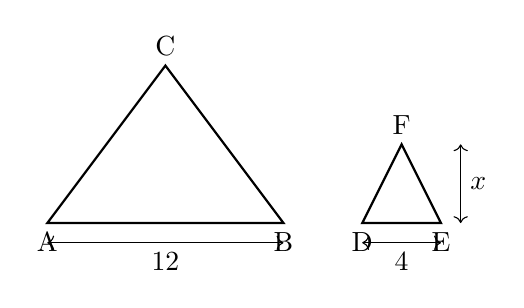
\begin{tikzpicture}[scale=0.5]
    \draw[thick] (0,0) -- (6,0) -- (3,4) -- cycle;
    \node[below] at (0,0) {A};
    \node[below] at (6,0) {B};
    \node[above] at (3,4) {C};
    \draw[<->] (0,-0.5) -- (6,-0.5) node[midway,below] {12};
    
    \draw[thick] (8,0) -- (10,0) -- (9,2) -- cycle;
    \node[below] at (8,0) {D};
    \node[below] at (10,0) {E};
    \node[above] at (9,2) {F};
    \draw[<->] (8,-0.5) -- (10,-0.5) node[midway,below] {4};
    \draw[<->] (10.5,0) -- (10.5,2) node[midway,right] {$x$};
    \end{tikzpicture}
    \end{center}
    
    \item Dois triângulos são semelhantes com razão 3:2. Se o perímetro do maior é 30 cm, qual o perímetro do menor?
    
    \item A área de um triângulo é 36 cm². Qual a área de um triângulo semelhante com lados 50\% maiores?
\end{enumerate}

\columnbreak

\section*{3. Teorema de Tales}

\begin{center}
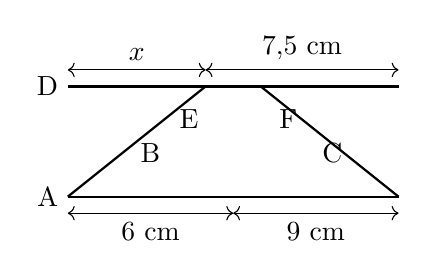
\begin{tikzpicture}[scale=0.7]
\draw[thick] (0,0) -- (6,0);
\draw[thick] (0,2) -- (6,2);
\draw[thick] (0,0) -- (2.5,2);
\draw[thick] (6,0) -- (3.5,2);
\node[left] at (0,0) {A};
\node[left] at (0,2) {D};
\node at (1.5,0.8) {B};
\node at (2.2,1.4) {E};
\node at (4.8,0.8) {C};
\node at (4,1.4) {F};
\draw[<->] (0,-0.3) -- (3,-0.3) node[midway,below] {6 cm};
\draw[<->] (3,-0.3) -- (6,-0.3) node[midway,below] {9 cm};
\draw[<->] (0,2.3) -- (2.5,2.3) node[midway,above] {$x$};
\draw[<->] (2.5,2.3) -- (6,2.3) node[midway,above] {7,5 cm};
\end{tikzpicture}
\end{center}

\[
\frac{AB}{BC} = \frac{DE}{EF} \quad \Rightarrow \quad \frac{6}{9} = \frac{x}{7,5}
\]

\section*{4. Triângulo Retângulo}

\begin{center}
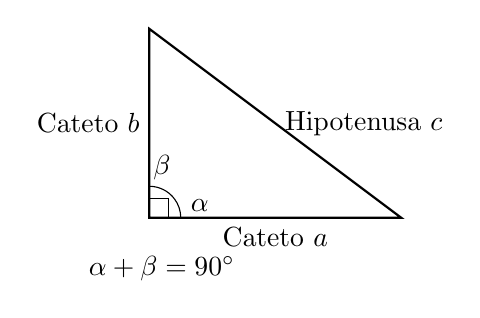
\begin{tikzpicture}[scale=0.8]
\draw[thick] (0,0) -- (4,0) -- (0,3) -- cycle;
\draw (0,0) rectangle (0.3,0.3);
\node[left] at (0,1.5) {Cateto $b$};
\node[below] at (2,0) {Cateto $a$};
\node[right] at (2,1.5) {Hipotenusa $c$};
\draw (0.5,0) arc (0:37:0.5);
\node at (0.8,0.2) {$\alpha$};
\draw (0,0.5) arc (90:37:0.5);
\node at (0.2,0.8) {$\beta$};
\node at (0.2,-0.8) {$\alpha + \beta = 90^\circ$};
\end{tikzpicture}
\end{center}

\subsection*{Teorema de Pitágoras}
\[
a^2 + b^2 = c^2
\]

\subsection*{Exercícios de Pitágoras}
\begin{enumerate}
    \item Calcule a hipotenusa:
    \begin{enumerate}[label=\alph*)]
        \item Catetos: 3 cm e 4 cm
        \item Catetos: 5 m e 12 m
        \item Catetos: 6 cm e 8 cm
    \end{enumerate}
    
    \item Calcule o cateto:
    \begin{enumerate}[label=\alph*)]
        \item Hipotenusa: 10 cm, cateto: 6 cm
        \item Hipotenusa: 13 m, cateto: 5 m
        \item Hipotenusa: 15 cm, cateto: 9 cm
    \end{enumerate}
\end{enumerate}

\section*{5. Relações Métricas no Triângulo Retângulo}

\begin{center}
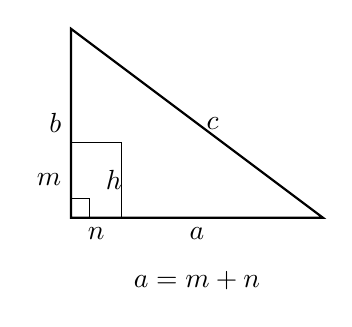
\begin{tikzpicture}[scale=0.8]
\draw[thick] (0,0) -- (4,0) -- (0,3) -- cycle;
\draw[dashed] (0,3) -- (0,0);
\draw (0,0) rectangle (0.3,0.3);
\node[below] at (2,0) {$a$};
\node[left] at (0,1.5) {$b$};
\node[right] at (2,1.5) {$c$};
\draw (0,1.2) -- (0.8,1.2) -- (0.8,0);
\node[left] at (0,0.6) {$m$};
\node[below] at (0.4,0) {$n$};
\node[right] at (0.4,0.6) {$h$};
\node at (2,-1) {$a = m + n$};
\end{tikzpicture}
\end{center}

\subsection*{Relações Métricas}
\begin{itemize}
    \item $b^2 = a \cdot m$
    \item $c^2 = a \cdot n$
    \item $h^2 = m \cdot n$
    \item $b \cdot c = a \cdot h$
    \item $\dfrac{1}{h^2} = \dfrac{1}{b^2} + \dfrac{1}{c^2}$
\end{itemize}

\subsection*{Exercícios de Relações Métricas}
\begin{enumerate}
    \item No triângulo retângulo, $a = 10$ cm, $m = 6$ cm. Calcule $b$, $c$, $h$ e $n$.
    \item Se $b = 12$ cm e $c = 16$ cm, calcule $h$.
    \item $m = 4$ cm, $n = 9$ cm. Calcule $h$, $b$, $c$ e $a$.
\end{enumerate}

\section*{6. Razões Trigonométricas}

\begin{center}
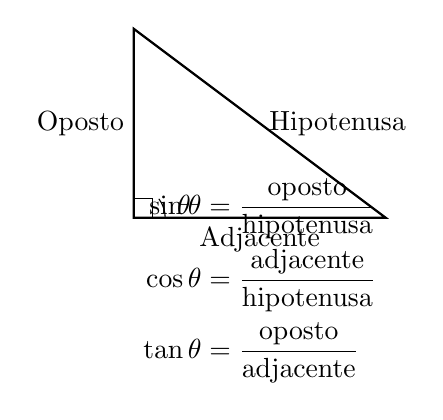
\begin{tikzpicture}[scale=0.8]
\draw[thick] (0,0) -- (4,0) -- (0,3) -- cycle;
\draw (0,0) rectangle (0.3,0.3);
\node[below] at (2,0) {Adjacente};
\node[left] at (0,1.5) {Oposto};
\node[right] at (2,1.5) {Hipotenusa};
\draw (0.5,0) arc (0:37:0.5);
\node at (0.8,0.2) {$\theta$};
\node at (2,-1) {
$\begin{aligned}
\sin\theta &= \frac{\text{oposto}}{\text{hipotenusa}} \\
\cos\theta &= \frac{\text{adjacente}}{\text{hipotenusa}} \\
\tan\theta &= \frac{\text{oposto}}{\text{adjacente}}
\end{aligned}$
};
\end{tikzpicture}
\end{center}

\subsection*{Razões Trigonométricas Fundamentais}
\[
\sin\theta = \frac{b}{a}, \quad \cos\theta = \frac{c}{a}, \quad \tan\theta = \frac{b}{c}
\]

\subsection*{Relação Fundamental}
\[
\sin^2\theta + \cos^2\theta = 1
\]

\subsection*{Ângulos Notáveis}
\begin{center}
\begin{tabular}{|c|c|c|c|}
\hline
Ângulo & $\sin$ & $\cos$ & $\tan$ \\
\hline
$30^\circ$ & $\frac{1}{2}$ & $\frac{\sqrt{3}}{2}$ & $\frac{\sqrt{3}}{3}$ \\
\hline
$45^\circ$ & $\frac{\sqrt{2}}{2}$ & $\frac{\sqrt{2}}{2}$ & 1 \\
\hline
$60^\circ$ & $\frac{\sqrt{3}}{2}$ & $\frac{1}{2}$ & $\sqrt{3}$ \\
\hline
\end{tabular}
\end{center}

\section*{7. Exercícios de Trigonometria}

\begin{enumerate}
    \item Calcule as razões trigonométricas:
    \begin{center}
    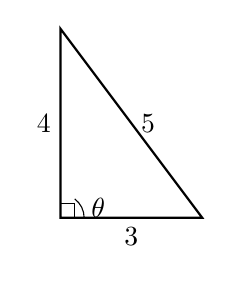
\begin{tikzpicture}[scale=0.6]
    \draw[thick] (0,0) -- (3,0) -- (0,4) -- cycle;
    \draw (0,0) rectangle (0.3,0.3);
    \node[below] at (1.5,0) {3};
    \node[left] at (0,2) {4};
    \node[right] at (1.5,2) {5};
    \draw (0.5,0) arc (0:53:0.5);
    \node at (0.8,0.2) {$\theta$};
    \end{tikzpicture}
    \end{center}
    \begin{enumerate}[label=\alph*)]
        \item $\sin\theta$
        \item $\cos\theta$
        \item $\tan\theta$
    \end{enumerate}
    
    \item Calcule usando ângulos notáveis:
    \begin{enumerate}[label=\alph*)]
        \item $\sin 30^\circ + \cos 60^\circ$
        \item $\tan 45^\circ - \sin 45^\circ$
        \item $2\cos 30^\circ + 3\sin 60^\circ$
    \end{enumerate}
    
    \item Aplicações:
    \begin{enumerate}[label=\alph*)]
        \item Uma escada de 5 m forma $60^\circ$ com o chão. Qual a altura da parede?
        \item Um avião está a 1000 m de altitude com ângulo de $30^\circ$. Qual a distância horizontal?
    \end{enumerate}
\end{enumerate}

\section*{8. Problemas Integrados}

\begin{enumerate}
    \item Na figura, calcule $x$:
    \begin{center}
    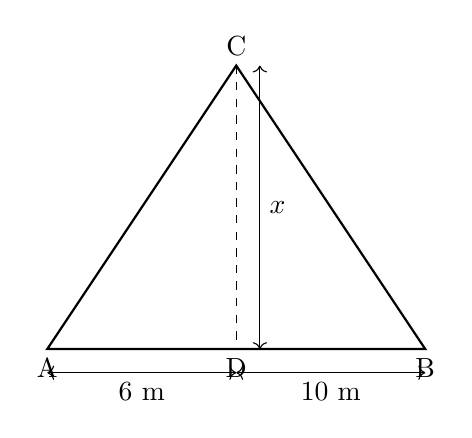
\begin{tikzpicture}[scale=0.6]
    \draw[thick] (0,0) -- (8,0) -- (4,6) -- cycle;
    \draw[dashed] (4,6) -- (4,0);
    \node[below] at (0,0) {A};
    \node[below] at (8,0) {B};
    \node[above] at (4,6) {C};
    \node[below] at (4,0) {D};
    \draw[<->] (0,-0.5) -- (4,-0.5) node[midway,below] {6 m};
    \draw[<->] (4,-0.5) -- (8,-0.5) node[midway,below] {10 m};
    \draw[<->] (4.5,0) -- (4.5,6) node[midway,right] {$x$};
    \end{tikzpicture}
    \end{center}
    
    \item Um poste de 8 m projeta sombra de 6 m. Qual o ângulo do sol com o horizonte?
    
    \item Dois triângulos são semelhantes. O maior tem lados 9 cm, 12 cm, 15 cm. O menor tem perímetro 18 cm. Calcule seus lados.
    
    \item Em um triângulo retângulo, $\sin\theta = 0,6$ e hipotenusa = 10 cm. Calcule os catetos.
    
    \item Prove que em triângulos semelhantes, a razão das áreas é o quadrado da razão de semelhança.
\end{enumerate}

\section*{9. Resumo das Fórmulas}

\subsection*{Congruência e Semelhança}
\begin{itemize}
    \item Casos LAL, ALA, LLL, LAA
    \item Razão de semelhança: $k = \frac{l_1}{l_2}$
    \item Razão de áreas: $k^2$
\end{itemize}

\subsection*{Triângulo Retângulo}
\begin{itemize}
    \item Pitágoras: $a^2 + b^2 = c^2$
    \item Relações métricas: $b^2 = a \cdot m$, $c^2 = a \cdot n$, $h^2 = m \cdot n$
    \item Trigonometria: $\sin = \frac{O}{H}$, $\cos = \frac{A}{H}$, $\tan = \frac{O}{A}$
    \item $\sin^2\theta + \cos^2\theta = 1$
\end{itemize}

\end{multicols}

\end{document}
